
\begin{frame}[t,allowframebreaks]{Gradient-based optimization -}


    Training a \gls{ml} model requires 
    some kind of \index{optimisation}\gls{optimisation}.
    \begin{itemize}
        \item Training is not a {\bf pure} \gls{optimisation} problem, 
        as we will discuss later. (See section on `\Gls{generalisation}'. 
        \hyperlink{sec:Generalisation}{\beamerbutton{link}})
    \end{itemize}
    \vspace{0.2cm}

    Often, we try to achieve the \index{extremisation}\gls{extremisation} 
    (minimisation or maximisation) of an 
    \index{objective function}\gls{objective function} or 
    \index{criterion}\gls{criterion}.
    \begin{itemize}
        \item 
            When the \gls{objective function} is minimised, 
            it is often called the
            \index{cost function}\gls{cost function},
            \index{loss function}\gls{loss function}, or
            \index{error function}\gls{error function}$^{(1)}$.
    \end{itemize}
    \vspace{0.2cm}
    The values extremising a function, 
    are often denoted with a $^\star$ superscript.
    So, if $f(\vect{x}): \mathbb{R}^n \rightarrow \mathbb{R}$ 
    is an \gls{objective function}
    we may write:
    \begin{equation*}
        \vect{x}^{\star} = \mathrm{argmin} \; f(\vect{x})
        \;\;\;\;\; \textrm{or} \;\;\;\;\;
        \vect{x}^{\star} = \mathrm{argmax} \; f(\vect{x})
    \end{equation*}

    \vspace{0.1cm}
    \noindent\rule{4cm}{0.4pt}\\
    {\tiny
    (1) Note that some authors assign subtle differences in these terms,
    while others use them interchangeably.\\
    }
    
    \framebreak

    %
    %

    Suppose $y=f(x)$ is a function whose domain and range is $\mathbb{R}$.\\
    \vspace{0.2cm}

    The \index{derivative}\gls{derivative} of $f(x)$, is another function 
    denoted as $f^\prime(x)$ or $df(x)/dx$.\\
    \vspace{0.3cm}
    
    The function $f^\prime(x)$:
    \begin{itemize}
        \item
        gives the {\bf slope of $f(x)$ at $x$} or, in other words,
        \item
        describes how to         
        scale a small change in the input $x$
        to compute a first-order approximation of the function $f$ at the new point:
        \begin{equation}
          f(x+\epsilon) \approx f(x) + \epsilon \; f^\prime(x)  
          \label{eq:deriv_1}
       \end{equation}\\
    \end{itemize}
    If $f(\vect{x})$
    is a scalar function of $n$ parameters,  
    the \index{gradient}\gls{gradient} $\nabla_{\vect{x}} f(\vect{x})$:
    \begin{equation}
        \nabla_{\vect{x}} f(\vect{x}) = 
        \Big( 
            \frac{\partial f(\vect{x})}{\partial x_1},
            \frac{\partial f(\vect{x})}{\partial x_2},
            \cdots ,
            \frac{\partial f(\vect{x})}{\partial x_n}
        \Big)
        \label{eq:gradient_1}
     \end{equation}\\
     generalises the concept of the \gls{derivative} in $n$-dimensional spaces.

    \framebreak

    %
    %

    {\bf The \index{gradient}\gls{gradient} $\nabla_{\vect{x}} f(\vect{x})$ 
    is useful for the 
    \index{extremisation}\gls{extremisation} of $f(\vect{x})$.}\\
    \vspace{0.2cm}
    \begin{itemize}
        \item
            It specifies how to make a small step in the space of $\vect{x}$, 
            in order to make a small improvement in $f(\vect{x})$ 
            in the desired direction.\\
            \vspace{0.1cm}
        \item
            Starting from a point $\vect{x}$, a calculation of 
            the \index{gradient}\gls{gradient} allows one to
            propose a new point $\vect{x}^\prime$ 
            on the path towards the function minimum$^{(1)}$:
            \begin{equation}
                \vect{x} \rightarrow \vect{x}^\prime = 
                    \vect{x} - \alpha \nabla_{\vect{x}} f(\vect{x})
                \label{eq:grad_descent_1}
            \end{equation}\\
            where $\alpha$ is a \index{hyperparameter}\gls{hyperparameter}
            controlling the \index{learning rate}\gls{learning rate}.
    \end{itemize}

    \vspace{0.1cm}

    This iterative \index{optimisation}\gls{optimisation} 
    technique is known as 
    \index{gradient}\index{gradient descent}{\bf \gls{gradient descent}}.
    \begin{itemize}
      \small
      \item The method is attributed to L.A. Cauchy (1847)
       \cite{Cauchy:GradientDescent}, who used it to solve systems of
       simultaneous equations that determine the orbits of stars.
    \end{itemize}

    \vspace{0.1cm}
    \noindent\rule{4cm}{0.4pt}\\
    {\tiny
    (1) Similarly, if we seek to maximise $f(\vect{x})$ 
    we move up the slope
    $\displaystyle \vect{x} \rightarrow \vect{x}^\prime =
      \vect{x} {\color{cadmiumred}+} \alpha \nabla_{\vect{x}} f(\vect{x})$.\\
    }

    \framebreak

    %
    %

    \vspace{-1.0cm}

    \begin{center}
        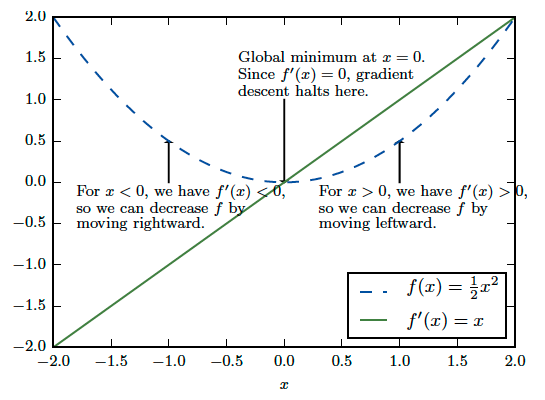
\includegraphics[width=0.80\textwidth]
            {./images/grad_descent/goodfellow17_grad_descent_1d.png}\\
        {\tiny 
            Simple illustration of the method of
            \index{gradient}\index{gradient descent}{\bf \gls{gradient descent}}.
            \color{col:attribution} 
            Schematic reproduced from p. 80 of \cite{Goodfellow:2017MITDL}.\\
        }
    \end{center}        

    \framebreak

    %
    %

    The \index{gradient}\index{gradient descent}\gls{gradient descent} method
    readily generalizes in multiple dimensions.\\


    \begin{columns}
        \begin{column}{0.80\textwidth}
            \begin{center}
                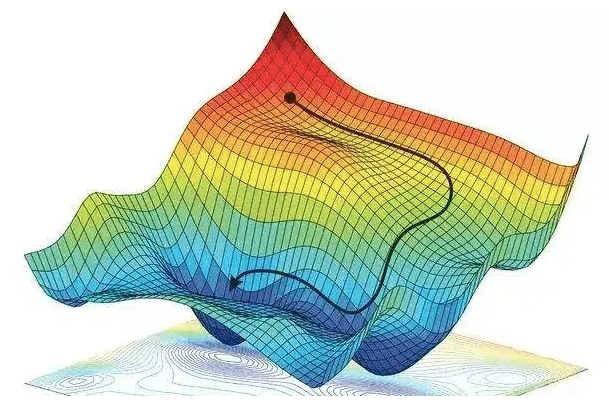
\includegraphics[width=0.99\textwidth]
                    {./images/grad_descent/guliyev20_grad_descent_2d.png}\\
                {\tiny 
                    Simple illustration of the method of
                    \index{gradient}\index{gradient descent}{\bf \gls{gradient descent}}.
                    \color{col:attribution} 
                    Schematic reproduced from \cite{Medium:GradDescentOptLinReg}.\\
                }
            \end{center}                    
        \end{column}
        \begin{column}{0.20\textwidth}
        {\scriptsize
            The method has several weaknesses when applied to
            optimization problems in multiple dimensions.\\
            \vspace{0.2cm}
            Later in this lecture, 
            we will discuss these weaknesses and 
            improved algorithms.\\
        
        }    
        \end{column}
    \end{columns}

    \framebreak

    %
    %

    There are various types of 
    \index{gradient}\index{gradient descent}{\bf \gls{gradient descent}}
    algorithms:\\
    \begin{itemize}
        \item   
            \index{batch gradient descent}
            \Gls{batch gradient descent}\\
            \begin{itemize}
                \item
                    Updates the model parameters 
                    after an iteration over all examples in the training set
                    (defining a training \index{epoch}\gls{epoch}).
            \end{itemize}
        \item 
            \index{mini batch gradient descent}
            \Gls{mini batch gradient descent}\\
            \begin{itemize}
                \item   
                    Separates the training set into small batches,
                    and updates the model parameters after an iteration
                    over all examples of each batch.
            \end{itemize}
        \item 
            \index{stochastic gradient descent}
            \Gls{stochastic gradient descent}\\
            \begin{itemize}
                \item   
                    Updates the model parameters after evaluating each
                    single example in the training set.\\
            \end{itemize}
    \end{itemize}

    \framebreak

    %
    %

    \vspace{-0.5cm}
    As we have seen, 
    \index{gradient}\index{gradient descent}\gls{gradient descent} 
    proposes a step (Eq.~\ref{eq:grad_descent_1}) 
    from $\vect{x}$ to $\vect{x}^\prime$:\\
    \vspace{-0.2cm}
    \begin{equation*}
        \vect{x} \rightarrow \vect{x}^\prime = 
            \vect{x} - \alpha \nabla_{\vect{x}} f(\vect{x})
    \end{equation*}\\
    \vspace{-0.1cm}
    The method is {\bf sensitive to the value of the 
    \index{learning rate}\gls{learning rate}, $\alpha$}.\\
    \begin{itemize}
        \small
        \item 
        If too large, the algorithm can 
        overshoot and step past the minimum.
        \item 
        If too small, the algorithm can become 
        too inefficient.
    \end{itemize}
    \begin{center}
        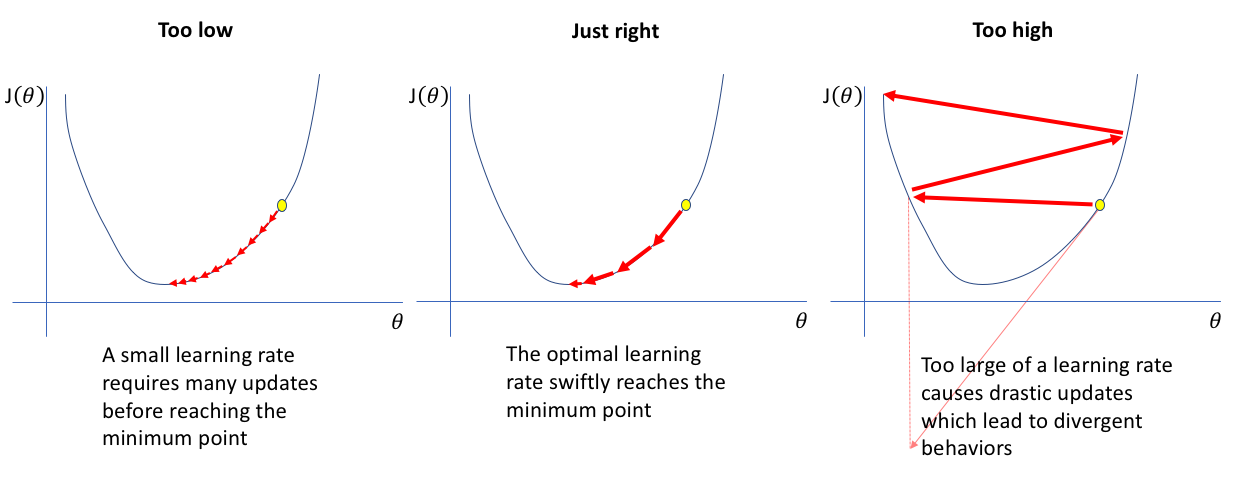
\includegraphics[width=0.88\textwidth]
            {./images/grad_descent/atu22_learning_rate_1.png}\\
        {\tiny 
            \color{col:attribution} 
            Schematic reproduced from \cite{Medium:GradDescent}.\\
        }
    \end{center}                    

    \framebreak

    %
    %

    There are several ways to choose the value of 
    the \index{learning rate}\gls{learning rate}, $\alpha$.\\
    \vspace{0.2cm}
    For example, we can:
    \begin{itemize}
        \item 
          set $\alpha$ to a small constant value,
        \item 
          solve for the value of $\alpha$ that makes the 
          directional derivative $\frac{\partial f(\vect{x})}{\partial \vect{n}}^{(1)}$ 
          vanish, i.e. move along $-\nabla_{\vect{x}} f(\vect{x})$
          till $f$ no longer descents, or
        \item 
          evaluate $f\big(\vect{x} - \alpha \nabla_{\vect{x}} f(\vect{x})\big)$
          for a range of $\alpha$ values, and  pick the one that leads to the smallest
          value of $f$ ({\bf line search} strategy).
    \end{itemize}
    \vspace{0.2cm}
    The choice impacts the {\bf efficient convergence} of the optimization.\\
    %\vspace{0.1cm}
    \noindent\rule{4cm}{0.4pt}\\
    \vspace{0.1cm}
    {\tiny
    (1) The directional derivative, 
    $\frac{\partial f(\vect{x})}{\partial \vect{n}}$,
    is the derivative of $f(\vect{x})$ in the direction of $\vect{\hat{n}}$. 
    It should not be confused with the gradient 
    $\nabla_{\vect{x}} f(\vect{x})$ though,
    clearly, they are connected: 
    $\frac{\partial f(\vect{x})}{\partial \vect{n}} = 
     \vect{n} \cdot \nabla_{\vect{x}} f(\vect{x})$.\\
    }


    \framebreak

    %
    %

    Points where the 
    \index{derivative}\gls{derivative} $f^\prime(x)$ 
    takes the value of 0  are known as 
    \index{critical point}\glspl{critical point} or 
    \index{stationary point}\glspl{stationary point}.\\

    \vspace{0.2cm}

    \begin{columns}
        \begin{column}{0.32\textwidth}
            These points are either: 
            \begin{itemize}
              \item \index{local minimum}\glspl{local minimum}, 
              \item \index{local maximum}\glspl{local maximum}, or
              \item \index{saddle point}\glspl{saddle point}.\\        
            \end{itemize}
            \end{column}
        \begin{column}{0.68\textwidth}

            \begin{center}
                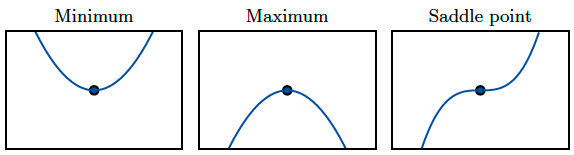
\includegraphics[width=0.80\textwidth]
                    {./images/grad_descent/goodfellow17_min_max_saddle_1d.png}\\
                {\tiny 
                    \color{col:attribution} 
                    Schematic reproduced from p. 81 of \cite{Goodfellow:2017MITDL}.\\
                }

                \vspace{0.6cm}

                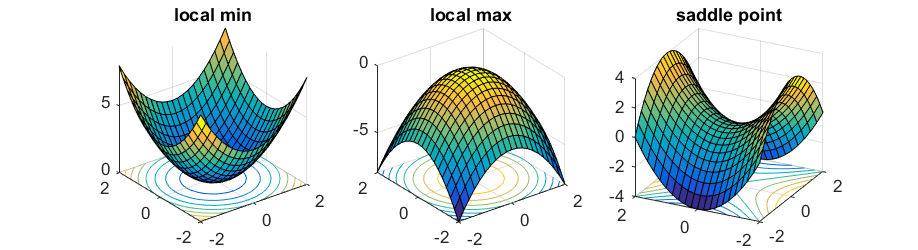
\includegraphics[width=0.99\textwidth]
                    {./images/grad_descent/ge16_min_max_saddle_2d.png}\\
                {\tiny 
                    \color{col:attribution} 
                    Schematic reproduced from \cite{OffConvex:EscapingSaddlePoints}.\\
                }
            \end{center}        
        
        \end{column}
    \end{columns}

\end{frame}


